\documentclass[tikz]{standalone}

\usepackage{tikz}
\usetikzlibrary{positioning, arrows.meta, shapes, snakes, shadings, calc}
\usepackage{amsmath,amssymb,amsthm,pgfplots}

\pgfmathdeclarefunction{gauss}{2}{%
  \pgfmathparse{1/(#2*sqrt(2*pi))*exp(-((x-#1)^2)/(2*#2^2))}
}

% polychrome colour, kelly
\definecolor{kwhite}{RGB}{242,243,244}
\definecolor{kred}{RGB}{175,35,55}
\definecolor{kyellow}{RGB}{236,195,66}
\definecolor{kblue}{RGB}{41,103,160}
\definecolor{kolivegreen}{RGB}{47,60,40}
\definecolor{kyellowgreen}{RGB}{150,180,55}
\definecolor{kpurplishpink}{RGB}{218,147,171}
\definecolor{korange}{RGB}{229,137,50}
\definecolor{kpurple}{RGB}{128,89,143}
\definecolor{kreddishbrown}{RGB}{126,51,31}
\definecolor{kgreen}{RGB}{59,133,90}
\definecolor{kbuff}{RGB}{192,178,134}
\definecolor{klightblue}{RGB}{169,201,237}
\definecolor{kyellowishpink}{RGB}{236,151,127}
\definecolor{kgrey}{RGB}{132,132,130}
\definecolor{kyellowishbrown}{RGB}{96,70,40}
\definecolor{kreddishorange}{RGB}{210,96,52}
\definecolor{kpurplishred}{RGB}{166,76,107}
\definecolor{kgreenishyellow}{RGB}{219,210,69}
\definecolor{korangeyellow}{RGB}{235,168,59}
\definecolor{kviolet}{RGB}{93,80,146}
\definecolor{kblack}{RGB}{34,34,34}
\definecolor{eedarkblue}{HTML}{202040}
\definecolor{eepurple}{HTML}{543864}
\definecolor{eered}{HTML}{ff6363}
\definecolor{eeyellow}{HTML}{ffbd69}
\definecolor{eecyan}{HTML}{64ccda}

\begin{document}
    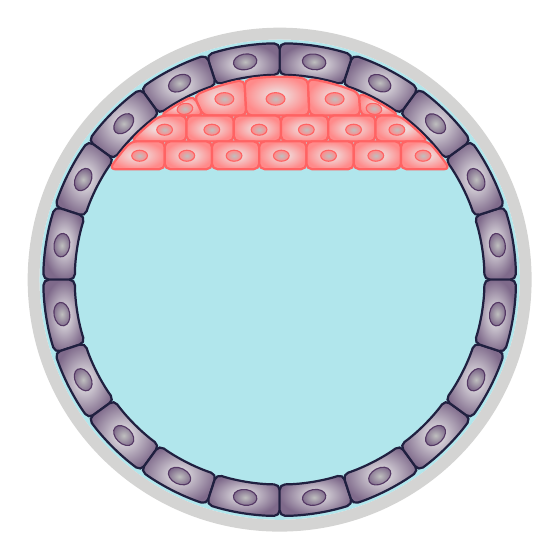
\begin{tikzpicture}[
        cyt/.style={thick, rounded corners=2pt, inner color=gray!15},
        nuc/.style={inner color=gray!50}
    ]
        % background
        \draw[draw=none, fill=eecyan!50] (0,0) circle[radius=3.05];
        
        % TE
        \foreach \x in {0,18,36,...,342}
        {
            \draw[cyt, draw=eedarkblue, outer color=eepurple!75, rotate around={\x:(0,0)}]
             (0:3) arc (0:18:3) -- (18:2.6) arc (18:0:2.6) -- cycle;
            \draw[nuc, draw=eepurple, outer color=eepurple!75, rotate around={\x:(0,0)}] (9:2.8) circle[x radius=0.1, y radius=0.15, rotate=10];
        }
        
        % ICM
        %% top row cells
        \draw[cyt, draw=eered, outer color=eered!75]
             (100:2.575) arc (100:115:2.575) -- (115:2.3) coordinate (tbl) -- +(0.55,0) coordinate (tbr) -- cycle;
        \draw[cyt, draw=eered, outer color=eered!75]
             (tbl) -- (126:2.575) arc (126:115:2.575) -- cycle;
        \draw[cyt, draw=eered, outer color=eered!75]
             (82:2.575) arc (82:100:2.575) -- (tbr) -- +(0.8,0) coordinate (tmr) -- cycle;
        \draw[cyt, draw=eered, outer color=eered!75]
             (67:2.575) arc (67:82:2.575) -- (tmr) -- +(0.65,0) coordinate (trr) -- cycle;
        \draw[cyt, draw=eered, outer color=eered!75]
             (67:2.575) arc (67:54:2.575) -- (trr) -- cycle;
        %% top row nuclei
        \draw[nuc, draw=eered, outer color=eered!75]
             (119:2.48) circle[x radius=0.1, y radius=0.07, rotate=10];
        \draw[nuc, draw=eered, outer color=eered!75]
             (107:2.4) coordinate (topnuc1) circle[x radius=0.12, y radius=0.08];
        \draw[nuc, draw=eered, outer color=eered!75]
             ($(topnuc1)+(0.65,0)$) circle[x radius=0.12, y radius=0.08];
        \draw[nuc, draw=eered, outer color=eered!75]
             ($(topnuc1)+(1.4,0)$) circle[x radius=0.12, y radius=0.08];
        \draw[nuc, draw=eered, outer color=eered!75]
             ($(119:2.48)+(2.4,0)$) circle[x radius=0.1, y radius=0.07, rotate=-10];
        %% middle row cells
        \draw[cyt, draw=eered, outer color=eered!75]
             (126:2.575) arc (126:137:2.575) -- +(0.7,0) coordinate (midb1) -- (midb1 |- tbl) coordinate (midu1) -- cycle;
        \draw[cyt, draw=eered, outer color=eered!75]
             (midb1) -- +(0.6,0) coordinate (midb2) -- (midb2 |- tbl) coordinate (midu2) -- (midu1) -- cycle;
        \draw[cyt, draw=eered, outer color=eered!75]
             (midb2) -- +(0.6,0) coordinate (midb3) -- (midb3 |- tbl) coordinate (midu3) -- (midu2) -- cycle;
        \draw[cyt, draw=eered, outer color=eered!75]
             (midb3) -- +(0.6,0) coordinate (midb4) -- (midb4 |- tbl) coordinate (midu4) -- (midu3) -- cycle;
        \draw[cyt, draw=eered, outer color=eered!75]
             (midb4) -- +(0.6,0) coordinate (midb5) -- (midb5|- tbl) coordinate (midu5) -- (midu4) -- cycle;
        \draw[cyt, draw=eered, outer color=eered!75]
             (midb5) -- (43:2.575) arc (43:54:2.575) -- (midu5) -- cycle;
        %% middle row nuclei
        \draw[nuc, draw=eered, outer color=eered!75]
             (127.5:2.4) coordinate (midnuc1) circle[x radius=0.1, y radius=0.07];
        \draw[nuc, draw=eered, outer color=eered!75]
             ($(midnuc1)+(0.6,0)$) circle[x radius=0.1, y radius=0.07];
        \draw[nuc, draw=eered, outer color=eered!75]
             ($(midnuc1)+(1.2,0)$) circle[x radius=0.1, y radius=0.07];
        \draw[nuc, draw=eered, outer color=eered!75]
             ($(midnuc1)+(1.8,0)$) circle[x radius=0.1, y radius=0.07];
        \draw[nuc, draw=eered, outer color=eered!75]
             ($(midnuc1)+(2.4,0)$) circle[x radius=0.1, y radius=0.07];
        \draw[nuc, draw=eered, outer color=eered!75]
             ($(midnuc1)+(2.95,0)$) circle[x radius=0.1, y radius=0.07];
        %% bottom row cells
        \draw[cyt, draw=eered, outer color=eered!75]
             (137:2.575) arc (137:147:2.575) -- +(0.7,0) coordinate (bb1) -- (bb1 |- midb1) coordinate (bu1) -- cycle;
        \draw[cyt, draw=eered, outer color=eered!75]
             (bb1) -- +(0.6,0) coordinate (bb2) -- (bb2 |- midb1) coordinate (bu2) -- (bu1) -- cycle;
        \draw[cyt, draw=eered, outer color=eered!75]
             (bb2) -- +(0.6,0) coordinate (bb3) -- (bb3 |- midb1) coordinate (bu3) -- (bu2) -- cycle;
        \draw[cyt, draw=eered, outer color=eered!75]
             (bb3) -- +(0.6,0) coordinate (bb4) -- (bb4 |- midb1) coordinate (bu4) -- (bu3) -- cycle;
        \draw[cyt, draw=eered, outer color=eered!75]
             (bb4) -- +(0.6,0) coordinate (bb5) -- (bb5 |- midb1) coordinate (bu5) -- (bu4) -- cycle;
        \draw[cyt, draw=eered, outer color=eered!75]
             (bb5) -- +(0.6,0) coordinate (bb6) -- (bb6 |- midb1) coordinate (bu6) -- (bu5) -- cycle;
        \draw[cyt, draw=eered, outer color=eered!75]
             (bb6) -- (33:2.575) arc (33:43:2.575) -- (bu6) -- cycle;
        %% bottom row nuclei
        \draw[nuc, draw=eered, outer color=eered!75]
             (138.5:2.375) coordinate (bnuc1) circle[x radius=0.1, y radius=0.07];
        \draw[nuc, draw=eered, outer color=eered!75]
             ($(bnuc1)+(0.6,0)$) circle[x radius=0.1, y radius=0.07];
        \draw[nuc, draw=eered, outer color=eered!75]
             ($(bnuc1)+(1.2,0)$) circle[x radius=0.1, y radius=0.07];
        \draw[nuc, draw=eered, outer color=eered!75]
             ($(bnuc1)+(1.8,0)$) circle[x radius=0.1, y radius=0.07];
        \draw[nuc, draw=eered, outer color=eered!75]
             ($(bnuc1)+(2.4,0)$) circle[x radius=0.1, y radius=0.07];
             \draw[nuc, draw=eered, outer color=eered!75]
             ($(bnuc1)+(3.0,0)$) circle[x radius=0.1, y radius=0.07];
             \draw[nuc, draw=eered, outer color=eered!75]
             ($(bnuc1)+(3.6,0)$) circle[x radius=0.1, y radius=0.07];
             
        % zona pellucida
        \draw[draw=none, fill=kgrey!35, even odd rule]
            (0,0) circle[radius=3.2] (0,0) circle[radius=3.05];
        
%        \draw[help lines, step=0.1] (-3,-3) grid (3,3);
    \end{tikzpicture}   
\end{document}